%# -*- coding:utf-8 -*-
\subsection[中心线提取]{基于Voronoi图的血管模型中心线的提取}

\begin{frame}
\begin{itemize}
  \item \textbf{表面模型中心线提取流程}:
\end{itemize}
\begin{figure}[t]
\centering
%# -*- coding:utf-8 -*-
\begin{tikzpicture}[scale=.3]

\draw [black,thick,rounded corners] (-3,0) rectangle (3,2);            % binary threshold
\draw [black,thick,rounded corners] (-3,3) rectangle (3,5);  % GAC

\draw [black,thick,rounded corners] (-8,7) rectangle (-2,9); % fast marching
\draw [black,thick,rounded corners] (-8,13) rectangle (-2,15); % thresholding
\draw [black,thin,dashed] (-8.5,6.5) rectangle (-1.5,15.5);
\node [above right] at (-8.5,15.5) {\tiny \fs \bf 初始水平集};

\draw [black,thick,rounded corners] (2,7) rectangle (8,9);   % sigmoid
\draw [black,thick,rounded corners] (2,10) rectangle (8,12); % gradient
\draw [black,thick,rounded corners] (2,13) rectangle (8,15); % curvature anisotropic diffusion
\draw [black,thin,dashed] (1.5,6.5) rectangle (8.5,15.5);
\node [above right] at (5,15.5) {\tiny \fs \bf 特征图像};

\draw [black,thick,rounded corners] (-3,17) rectangle (3,19); % raw input

\node [above right] at (-2.1,0.25) {\tiny \fs \bf 二值阈值滤波};
\node [above right] at (-2.1,3.25) {\tiny \fs \bf 测地活动轮廓};

\node [above right] at (-6.75,7.25) {\tiny \fs \bf 快速行进};
\node [above right] at (-6.75,13.25) {\tiny \fs \bf 阈值滤波};

\node [above right] at (2.3,7.25) {\tiny \fs \bf 亮度的非线性映射};
\node [above right] at (3,10.25) {\tiny \fs \bf 梯度幅值计算};
\node [above right] at (2.3,13.25) {\tiny \fs \bf 曲率各向异性扩散};

\node [above right] at (-1.9,17.25) {\tiny \fs \bf 原始体数据};

\draw [<-,thick] (0,2) -- (0,3);

\draw [<-,thick] (0,5) -- (0,6);
\draw [thick] (-5,6) -- (5,6);
\draw [thick] (-5,6) -- (-5,7);
\draw [thick] (5,6) -- (5,7);

\draw [<-,thick] (-5,9) -- (-5,13);
\draw [<-,thick] (5,9) -- (5,10);

\draw [<-,thick] (5,9) -- (5,10);
\draw [<-,thick] (5,12) -- (5,13);

\draw [<-,thick] (-5,15) -- (-5,16);
\draw [<-,thick] (5,15) -- (5,16);
\draw [thick] (-5,16) -- (5,16);
\draw [thick] (0,16) -- (0,17);

\end{tikzpicture} 
% 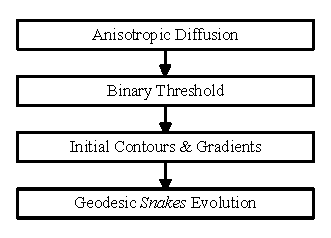
\includegraphics[width=3.2in]{Figures/gac/DataFlow.eps}
% \caption[主动脉内腔分割流程]{主动脉内腔分割流程。}
% \label{fig:aorta_data_flow}
\end{figure}
\end{frame}

\begin{frame}
\begin{itemize}
  \item \textbf{区段模型及其顶点连接性验证}:
  \begin{itemize}
    \item 主动脉下半段表面模型(由$205,590$个多边形构成)与VOI提取的模型局部(红色方框内)
    \item 所提取区段血管表面模型的连接性验证结果(多边形面片数量:$70,625$)
  \end{itemize}
\end{itemize}
\begin{columns}[b,onlytextwidth]
\begin{column}{.5\textwidth}
\begin{figure}[t]
\centering
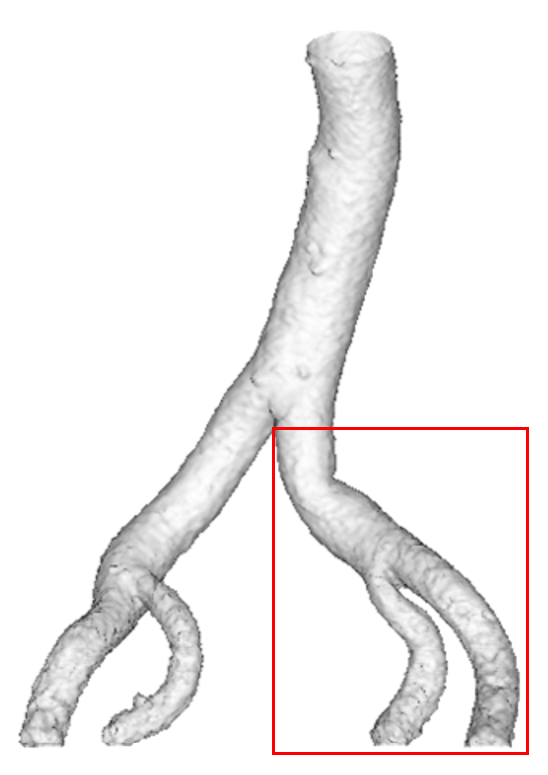
\includegraphics[height=1.5in]{../../Figures/postprocessing/centerlines/VOI.eps}
\end{figure}
\end{column}
\begin{column}{.5\textwidth}
\begin{figure}[t]
\centering
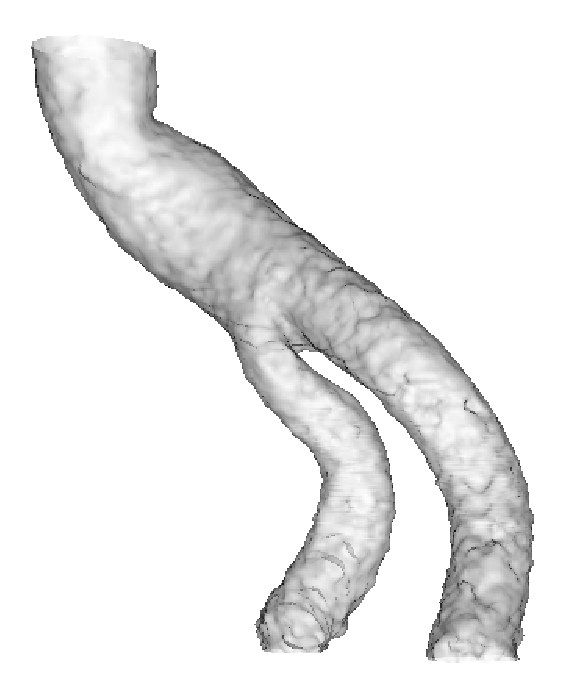
\includegraphics[height=1.5in]{../../Figures/postprocessing/centerlines/connectivity_local.eps}
\end{figure}
\end{column}
\end{columns}
\end{frame}

\begin{frame}
\begin{itemize}
  \item \textbf{连接性检验前后的多边形数量}:
  \begin{enumerate}[(a)]
    \item 本章实验数据
    \item 完整的血管模型
  \end{enumerate}
\end{itemize}
\begin{table}[!ht]
\renewcommand{\arraystretch}{0.5}
% \caption[连接性检验前后的多边形数量]{连接性验证前后多边形的数量:(a) 本章实验数据;(b) 完整的血管模型。}
% \label{tbl:centerlins_connectivity}
\centering
\begin{columns}[b,onlytextwidth]
\begin{column}{.5\textwidth}
\begin{tabular*}{40mm}{lc}
\toprule
~                                & \small{多边形数量} \\
\midrule
\small{验证前}                   & \small{$70,625$}  \\
\midrule
\small{验证后}                   & \small{$70,625$}  \\
\bottomrule
\end{tabular*}
\end{column}
\begin{column}{.5\textwidth}
\begin{tabular*}{40mm}{lc}
\toprule
~                                & \small{多边形数量} \\
\midrule
\small{验证前}                   & \small{$205,590$}  \\
\midrule
\small{验证后}                   & \small{$205,452$}  \\
\bottomrule
\end{tabular*}
\end{column}
\end{columns}
\end{table}
\end{frame}

\begin{frame}
\begin{itemize}
  \item \textbf{设置不同参数获得的平滑结果(中心线)}:
\end{itemize}
\begin{figure}[t]
% \begin{table}[t]
\renewcommand{\arraystretch}{0.5}
% \caption[为平滑算法设置不同的参数所获得的结果]{为平滑算法设置不同的参数所获得的结果($N$:迭代次数;$\delta$:带宽)}
% \label{tbl:mesh_smooth}
\centering
\begin{tabular}{|c|c|c|}
\hline
\bigstrut ~                                   & \raisebox{-1mm}{$N = 30$}                                                                     & \raisebox{-1mm}{$N = 100$}                                                  \\
\hline
\bigstrut[t] \raisebox{0mm}{$\delta = 0.1$}  & \Includegraphics[height=1.0in]{../../Figures/postprocessing/centerlines/smooth_30_1_local.eps}  & \Includegraphics[height=1.0in]{../../Figures/postprocessing/centerlines/smooth_30_01_local.eps}  \\
\hline
\bigstrut[b] \raisebox{0mm}{$\delta = 0.01$} & \Includegraphics[height=1.0in]{../../Figures/postprocessing/centerlines/smooth_100_1_local.eps} & \Includegraphics[height=1.0in]{../../Figures/postprocessing/centerlines/smooth_100_01_local.eps} \\
\hline
\end{tabular}
% \caption[设置不同参数获得的平滑结果(中心线)]{设置不同参数获得的平滑结果。($N$:迭代次数;$\delta$:带宽)}
% \label{fig:centerlines_smooth}
% \end{table}
\end{figure}
\end{frame}

\begin{frame}
\begin{itemize}
  \item \textbf{对平整后表面进行细分}:
  \begin{itemize}
    \item 左:表面细分的局部
    \item 右上:表面细分之前的多边形表面
    \item 右下:表面细分之后的多边形表面
  \end{itemize}
\end{itemize}
\begin{figure}[t]
\centering
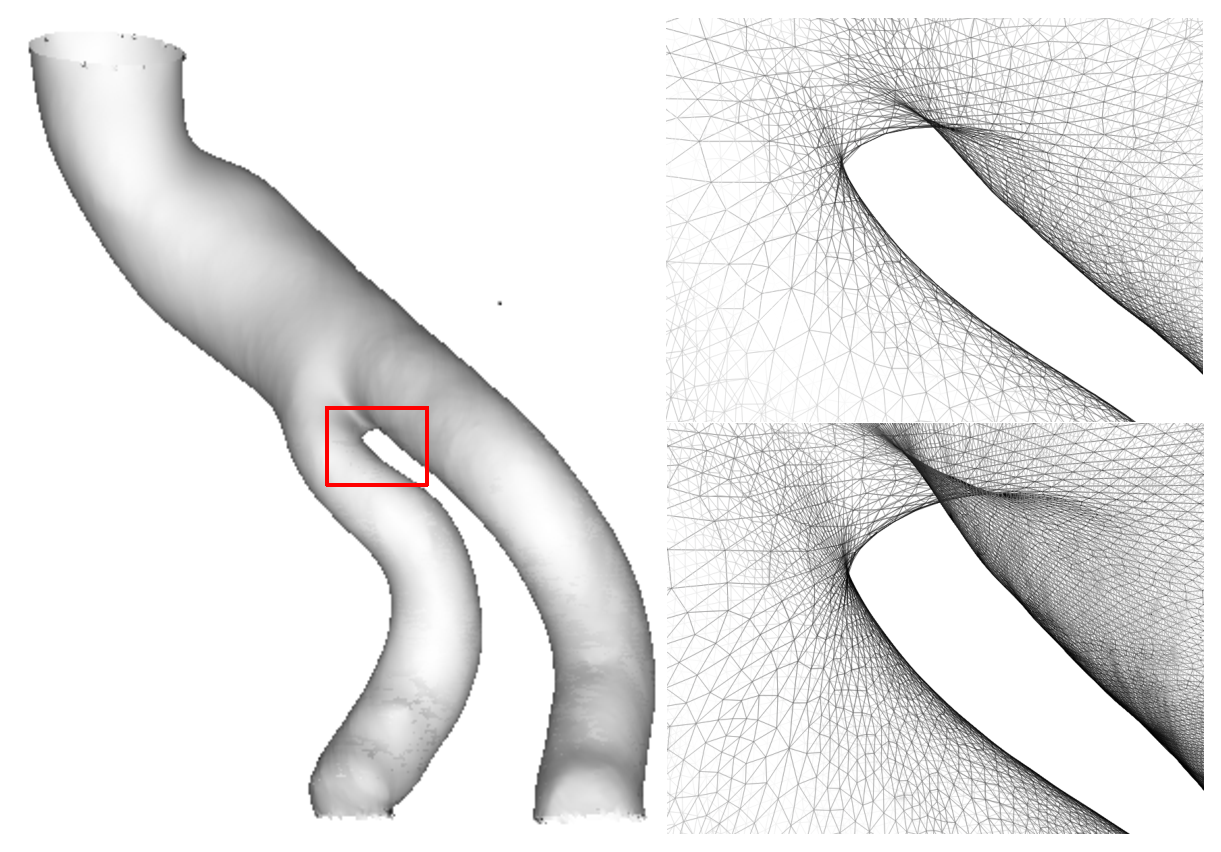
\includegraphics[height=1.5in]{../../Figures/postprocessing/centerlines/subdivision.eps}
% \caption[对平整后表面进行细分]{对平整后表面进行细分。左:表面细分的局部。右上:表面细分之前的多边形表面。右下:表面细分之后的多边形表面。}%
% \label{fig:centerlins_subdivision_local}
\end{figure}
\end{frame} 

\begin{frame}
\begin{itemize}
  \item \textbf{表面细分前后多边形数量对比}:
  \begin{enumerate}[(a)]
    \item 本章实验数据
    \item 完整的血管模型
  \end{enumerate}
\end{itemize}
\begin{table}[t]
\renewcommand{\arraystretch}{0.5}
% \caption[表面细分前后多边形数量对比]{表面细分前后多边形数量对比。(a) 本章实验数据;(b) 完整的血管模型。}
% \label{tbl:centerlins_subdivision}
\centering
\begin{columns}[b,onlytextwidth]
\begin{column}{.5\textwidth}
\begin{tabular*}{40mm}{lr}
\toprule
~              & \small{多边形数量} \\
\midrule
\small{细分前} & \small{$70,625$}     \\
\midrule
\small{细分后} & \small{$281,060$}    \\
\bottomrule
\end{tabular*}
\end{column}
\begin{column}{.5\textwidth}
\begin{tabular*}{40mm}{lr}
\toprule
~              & \small{多边形数量} \\
\midrule
\small{细分前} & \small{$205,452$}    \\
\midrule
\small{细分后} & \small{$821,808$}    \\
\bottomrule
\end{tabular*}
\end{column}
\end{columns}
\end{table}
\end{frame} 

\begin{frame}
\begin{itemize}
  \item \textbf{不同区段模型的中心线提取结果}
\end{itemize}
\begin{figure}[t]
% \begin{table}[t]
\renewcommand{\arraystretch}{0.5}
% \caption[为平滑算法设置不同的参数所获得的结果]{为平滑算法设置不同的参数所获得的结果($N$:迭代次数;$\delta$:带宽)}
% \label{tbl:mesh_smooth}
\centering
\begin{tabular}{|c|c|c|}
\hline
\bigstrut ~                                  & \raisebox{-1mm}{Voronoi图}                                                                     & \raisebox{-1mm}{中心线}                                                  \\
\hline
\bigstrut[t] \raisebox{0mm}{本章实验模型}  & \Includegraphics[height=1.0in]{../../Figures/postprocessing/centerlines/overlay_100_01_voronoi_local.eps}  & \Includegraphics[height=1.0in]{../../Figures/postprocessing/centerlines/overlay_100_01_centerlines_local.eps}  \\
\hline
\bigstrut[b] \raisebox{0mm}{主动脉下半段} & \Includegraphics[height=1.0in]{../../Figures/postprocessing/centerlines/overlay_100_01_voronoi.eps} & \Includegraphics[height=1.0in]{../../Figures/postprocessing/centerlines/overlay_100_01_centerlines.eps} \\
\hline
\end{tabular}
% \raisebox{45mm}{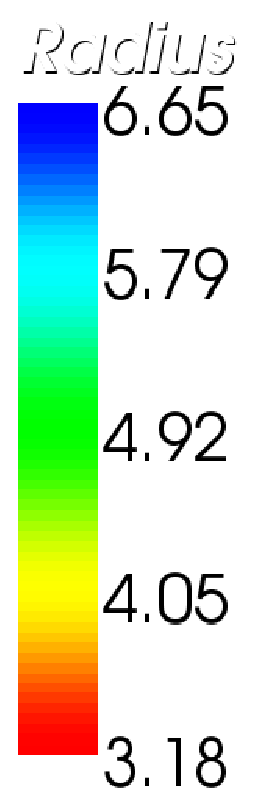
\includegraphics[height=1.0in,width=0.2in]{Figures/postprocessing/centerlines/scalarbar.eps}}
% \raisebox{-45mm}{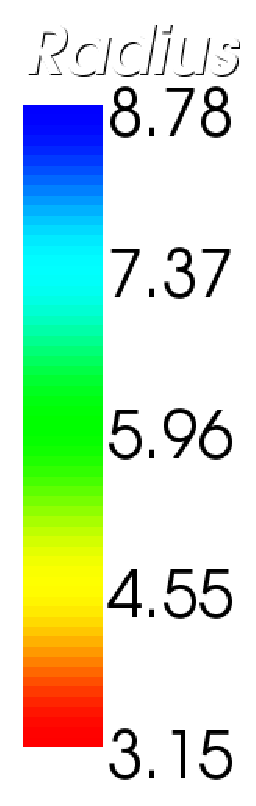
\includegraphics[width=0.2in]{Figures/postprocessing/centerlines/scalarbar2.eps}}
\raisebox{-20mm}{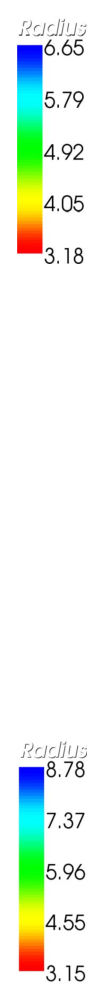
\includegraphics[height=1.5in]{../../Figures/postprocessing/centerlines/scalarbar12.eps}}
% \caption[不同区段模型的中心线提取结果]{不同区段模型的中心线提取结果。}
% \label{fig:centerlines}
% \end{table}
\end{figure}
\end{frame} 

\begin{frame}
\begin{itemize}
  \item \textbf{中心线计算时间}
\end{itemize}
\begin{table}[!ht]
\renewcommand{\arraystretch}{0.5}
% \caption[中心线计算时间]{中心线计算时间}
% \label{tbl:centerlins_computation_time}
\centering
\begin{tabular*}{55mm}{lr}
\toprule
~                                & \small{耗费时间(s)} \\
\midrule
\small{本章实验模型}             & \small{$780$}  \\
\midrule
\small{主动脉下半段}             & \small{$2,760$}  \\
\bottomrule
\end{tabular*}
\end{table}
\end{frame} 

\begin{frame}
\begin{itemize}
  \item \textbf{完整主动脉模型的中心线}:
  \begin{itemize}
    \item 基于CTA的表面模型(多边形的数量:$757,538$)
    \item 表面模型的中心线
  \end{itemize}
\end{itemize}
\begin{columns}[b,onlytextwidth]
\begin{column}{.5\textwidth}
\begin{figure}[t]
\centering
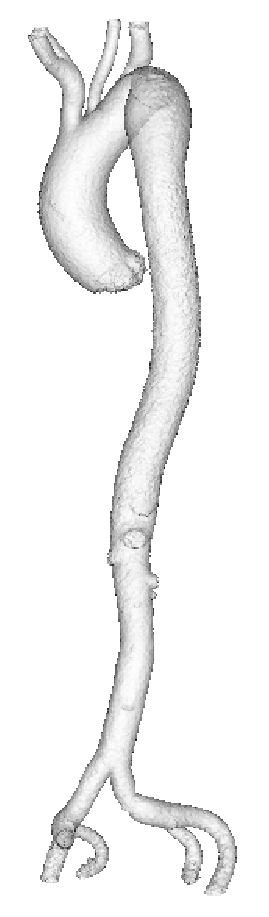
\includegraphics[height=1.5in]{../../Figures/postprocessing/centerlines/surface.eps}
\end{figure}
\end{column}
\begin{column}{.5\textwidth}
\begin{figure}[t]
\centering

\includegraphics[height=1.5in]{../../Figures/postprocessing/centerlines/centerlines.eps}
\end{figure}
\end{column}
\end{columns}
\end{frame}